\documentclass{article}
\usepackage{physics}
\usepackage{graphicx}
\usepackage{caption}
\usepackage{amsmath}
\usepackage{bm}
\usepackage{framed}
\usepackage{authblk}
\usepackage{empheq}
\usepackage{amsfonts}
\usepackage{esint}
\usepackage[makeroom]{cancel}
\usepackage{dsfont}
\usepackage{centernot}
\usepackage{mathtools}
\usepackage{bigints}
\usepackage{amsthm}
\theoremstyle{definition}
\newtheorem{defn}{Definition}[section]
\newtheorem{prop}{Proposition}[section]
\newtheorem{rmk}{Remark}[section]
\newtheorem{thm}{Theorem}[section]
\newtheorem{exmp}{Example}[section]
\newtheorem{prob}{Problem}[section]
\newtheorem{sln}{Solution}[section]
\newtheorem*{prob*}{Problem}
\newtheorem{exer}{Exercise}[section]
\newtheorem*{exer*}{Exercise}
\newtheorem*{sln*}{Solution}
\usepackage{empheq}
\usepackage{tensor}
\usepackage{xcolor}
%\definecolor{colby}{rgb}{0.0, 0.0, 0.5}
\definecolor{MIT}{RGB}{163, 31, 52}
\usepackage[pdftex]{hyperref}
%\hypersetup{colorlinks,urlcolor=colby}
\hypersetup{colorlinks,linkcolor={MIT},citecolor={MIT},urlcolor={MIT}}  



\newcommand*\widefbox[1]{\fbox{\hspace{2em}#1\hspace{2em}}}

\newcommand{\p}{\partial}
\newcommand{\R}{\mathbb{R}}
\newcommand{\C}{\mathbb{C}}
\newcommand{\lag}{\mathcal{L}}
\newcommand{\nn}{\nonumber}
\newcommand{\ham}{\mathcal{H}}
\newcommand{\M}{\mathcal{M}}
\newcommand{\I}{\mathcal{I}}
\newcommand{\K}{\mathcal{K}}
\newcommand{\F}{\mathcal{F}}
\newcommand{\w}{\omega}
\newcommand{\lam}{\lambda}
\newcommand{\al}{\alpha}
\newcommand{\be}{\beta}
\newcommand{\x}{\xi}

\newcommand{\G}{\mathcal{G}}

\newcommand{\f}[2]{\frac{#1}{#2}}

\newcommand{\ift}{\infty}

\newcommand{\lp}{\left(}
\newcommand{\rp}{\right)}

\newcommand{\lb}{\left[}
\newcommand{\rb}{\right]}

\newcommand{\lc}{\left\{}
\newcommand{\rc}{\right\}}


\newcommand{\V}{\mathbf{V}}
\newcommand{\U}{\mathcal{U}}
\newcommand{\Id}{\mathcal{I}}
\newcommand{\D}{\mathcal{D}}
\newcommand{\Z}{\mathcal{Z}}

%\setcounter{chapter}{-1}






\usepackage{subfig}
\usepackage{listings}
\captionsetup[lstlisting]{margin=0cm,format=hang,font=small,format=plain,labelfont={bf,up},textfont={it}}
\renewcommand*{\lstlistingname}{Code \textcolor{violet}{\textsl{Mathematica}}}
\definecolor{gris245}{RGB}{245,245,245}
\definecolor{olive}{RGB}{50,140,50}
\definecolor{brun}{RGB}{175,100,80}

%\hypersetup{colorlinks,urlcolor=colby}
\lstset{
	tabsize=4,
	frame=single,
	language=mathematica,
	basicstyle=\scriptsize\ttfamily,
	keywordstyle=\color{black},
	backgroundcolor=\color{gris245},
	commentstyle=\color{gray},
	showstringspaces=false,
	emph={
		r1,
		r2,
		epsilon,epsilon_,
		Newton,Newton_
	},emphstyle={\color{olive}},
	emph={[2]
		L,
		CouleurCourbe,
		PotentielEffectif,
		IdCourbe,
		Courbe
	},emphstyle={[2]\color{blue}},
	emph={[3]r,r_,n,n_},emphstyle={[3]\color{magenta}}
}


\begin{document}
	

\begin{center}
	\Large{Landau-Zener Transition Probability\\
	Notes and A Simple Numerical Verification}
\end{center}	
	
\begin{center}
	\large{Huan Q. Bui}
\end{center}

\begin{center}
	\today
\end{center}


\section{Avoided Crossing}

Recall results from avoided crossing: Given a Hamiltonian of the form 
\begin{equation*}
\widehat{H}' = \widehat{H} + \widehat{P} = \begin{bmatrix}
E_1 & \\ & E_2
\end{bmatrix} + \begin{bmatrix}
& E_{12} \\ E_{12}* &
\end{bmatrix} = \begin{bmatrix}
E_1 & E_{12} \\ E_{12}^* & E_2
\end{bmatrix},
\end{equation*}
the eigen-energies are
\begin{equation*}
E_\pm = \f{1}{2}(E_1 + E_2) \pm  \f{1}{2}\sqrt{(E_1 - E_2)^2 + 4\abs{E_{12}}^2}.
\end{equation*}
The avoided crossing is shown by plotting the energies $E_\pm$ against the zero-perturbation energy splitting $\Delta E = E_1 - E_2$. Now, imagine that this $\Delta$ is a function of time, then $\Delta E = \Delta E(t)$. In this case we can plot $E_\pm$ against time, and the result looks something like this:

\begin{figure}[!htb]
	\centering
	\includegraphics[width=0.75\textwidth]{avoided-crossing.png}
	\caption{Avoided crossing following Landau-Zener approximations.}
	\label{fig:LZ}
\end{figure}

In this simple system, two things can happen as we sweep $\Delta E$ (in time).  On the one hand, if we sweep very slowly (adiabatic), then eigenstates have time to ``adapt'' and remain at their relative energy levels, i.e., the lower-energy eigenstate will change its wavefunction so that its energy remains the lower energy, and vice versa. If we sweep very quickly (non-adiabatic), on the other hand, then the eigenstate may remain the same, with some probability of transitioning to other eigenstate(s). \\


What we mean by ``slowly'' and ``quickly'' is captured by the only two time scales in this problem: how fast we sweep the energy splitting and the rate of Rabi oscillation. It turns out that the adiabatic condition is given by 
\begin{equation*}
\f{\abs{E_{12}}}{\abs{\al}} \f{\abs{E_{12}}}{\hbar} = \f{\abs{E_{12}}^2}{\hbar\abs{\al}} \equiv \gamma \gg 1.
\end{equation*}

The main point here is that the transition probability mentioned above is called the Landau-Zener transition probability, named after two physicists who stated and solved the problem (analytically). As we will see below, this probability is an exponential decay which depends on the sweeping rate (how slowly/quickly $\Delta E$ changes) and how strong the two states are coupled. 


\section{Results for Linear LZ Sweep}

We will write the Hamiltonian with (possible) time dependence:
\begin{equation*}
\widehat{H} = \begin{bmatrix}
E_1(t) & E_{12}(t) \\ E_{12}(t)^* & E_{2}(t).
\end{bmatrix}
\end{equation*}



Landau and Zener's analytical solution arrived after making the following approximations and simplifications: 
\begin{itemize}
	\item $E_{12}$ is very small compared to $\Delta E$. We can treat it as constant.
	\item $\Delta E$ varies linearly in time 
\end{itemize}

From these simplifications we have, for all time, 
\begin{equation*}
\f{d}{dt}(E_1(t) - E_2(t)) = \al t \quad \text{ and } \quad \f{d}{dt}{E_{12}(t)} = 0.
\end{equation*}

To state the transition probability due to Landau and Zener, we must define it first. To this end, we first define the ``non-adiabatic'' basis by 
\begin{equation*}
\ket{1} = \begin{pmatrix}
1 \\ 0
\end{pmatrix} \quad \text{ and }  \quad
\ket{2} = \begin{pmatrix}
0 \\ 1
\end{pmatrix}
\end{equation*}

Next, let $\ket{\Psi(t)}$ solve the SE, then a natural ansatz for $\ket{\Psi(t)}$ is 
\begin{equation*}
\ket{\Psi(t)} = A(t) \exp \lp -\f{i}{\hbar}\int_0^{t} E_1(t')\,dt' \rp \ket{1} + B(t) \exp \lp -\f{i}{\hbar}\int_0^{t} E_2(t')\,dt' \rp \ket{2}.
\end{equation*}
We assume that at time $t=-\infty$, the system is in state $\ket{2}$, so that
\begin{equation*}
A(-\infty) = 0 \quad \text{ and } \quad B(-\infty) = 1.
\end{equation*}
We wish to find the probability $P$ that the system makes a transition from state $\ket{2}$ to $\ket{1}$, which is given by 
\begin{equation*}
P = \abs{B(\infty)}^2 = 1- \abs{A(\infty)}^2.
\end{equation*}
In his paper \cite{zener1932non}, Zener showed that 
\begin{equation*}
\boxed{P = e^{-2\pi \gamma}, \text{ where } \gamma = \f{\abs{E_{12}}^2}{\hbar \abs{\al}}} 
\end{equation*}
The derivation is quite nice. Zener casts the differential equation for $B(t)$ into the form of the \textbf{Weber's equation} and extracted the asymptotic behavior for $B(t)$ from there. 


\subsection{Numerical verification}



Since the (analytical) derivation of the Landau-Zener transition probability is rather involved, we will only work with a numerical verification. This verification is inspired by Problem set 7 of MIT's 8.06: Quantum Physics III - Spring 2018. \\


We start by getting a set of ODEs for $A(t)$ and $B(t)$ from the SE:
\begin{align*}
i\hbar  \f{d}{dt}A(t) &= E_{12} B(t)  \exp\lp -\f{i}{\hbar} \int_0^t E_2(t') - E_1(t') \,dt'\rp\\
i\hbar  \f{d}{dt}B(t) &= E_{12}^* A(t)  \exp\lp +\f{i}{\hbar} \int_0^t E_2(t') - E_1(t') \,dt'\rp
\end{align*}
Let $E_1(t) - E_2(t) = \Delta E(t)$, then 
\begin{align*}
i\hbar  \f{d}{dt}A(t) &= E_{12} B(t)  \exp\lp +\f{i}{\hbar} \int_0^t \Delta E(t') \,dt'\rp\\
i\hbar  \f{d}{dt}B(t) &= E_{12}^* A(t)  \exp\lp -\f{i}{\hbar} \int_0^t \Delta E(t') \,dt'\rp
\end{align*}
This is a set of linear, first-order, coupled DEs. From here, we can get a second-order DE for $B$. To get a nice, unit-free equation, we let
\begin{equation*}
\tau = \f{\al}{\abs{E_{12}}} t \quad \text{ and } \quad \gamma = \f{\abs{E_{12}}^2}{\hbar \al}.
\end{equation*}
We then get
\begin{equation*}
\f{d^2 B}{d\tau^2} + i\gamma \tau \f{dB}{d\tau} + \gamma^2 B = 0.
\end{equation*}

We will solve this for $\gamma = 0.1$ and $\tau \in [-60, 60]$. MATLAB code for this: 
\begin{lstlisting}
% Huan Q. Bui
% 2nd order ODE solver for Landau-Zener problem

clear all
close all
global gamma

tspan = [-60 60];
B0 = 1;
C0 = 0;
gamma = 0.1;

[t,y] = ode45(@LZ_ODE,tspan,[B0; C0]);
% y(1) = B
% y(2) = C = \dot{B}

plot(t,abs(y(:,1)).^2,'LineWidth', 2)
title('|B(t)|^2 with \gamma = 0.1 using ODE45');
xlabel('Time t');
ylabel('|B(t)|^2');
grid on

% plot LZ prediction
yline(exp(-2*pi*gamma), 'LineWidth',2);

% legend
legend('|B(t)|^2', 'Exp(-2\pi\gamma)');

function dydt = LZ_ODE(t,y)
global gamma
dydt = [y(2); -1i*gamma.*t.*y(2) - gamma^2.*y(1)];
end

\end{lstlisting}



Plotting $\abs{B(\tau)}$ against $\tau$ and plotting the predicted $\exp(-2\pi \gamma) = \lim_{\tau\to\infty}\abs{B(\tau)}^2$, we find good agreement:
\begin{figure}[!htb]
	\centering
	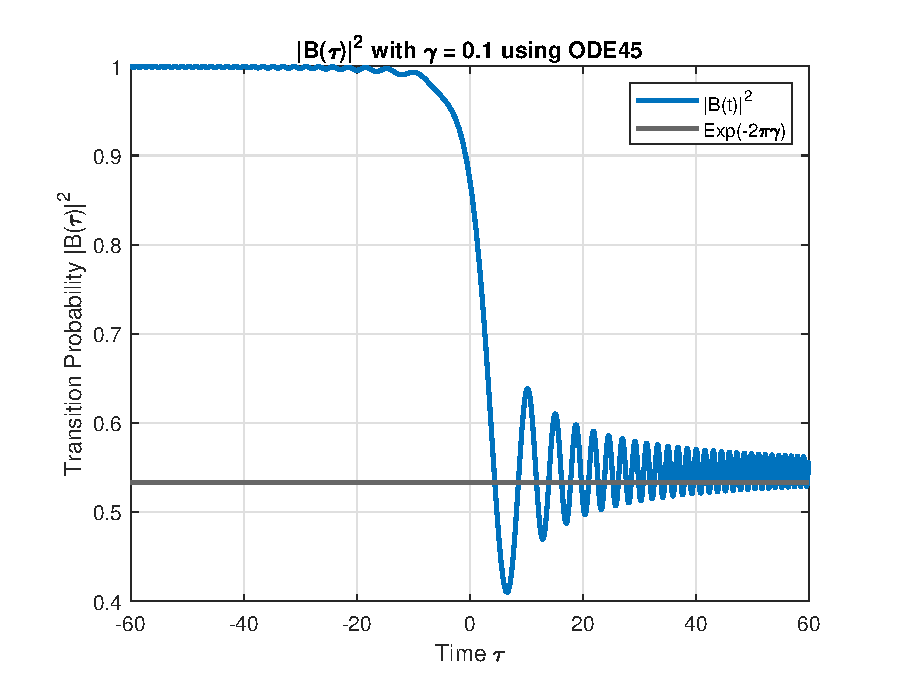
\includegraphics[width=0.75\textwidth]{LZ}
\end{figure}


We next test how well things agree by solving the ODE in $B(t)$ for a range of $\gamma$'s. We expect that as the time span of the solver is increased, $\abs{B(t_{\text{final}})}^2$ approach $\exp(-2\pi \gamma)$ better and better. See Figure \ref{fig:tau_Infty}.

\begin{figure}[!htb]
	\begin{minipage}{0.49\textwidth}
		\centering
		\includegraphics[width=\textwidth]{t050.eps}
		\caption{$\tau\in [-50,50]$}
		\includegraphics[width=\textwidth]{t100.eps}
		\caption{$\tau\in [-100,100]$}
	\end{minipage}
	\begin{minipage}{0.49\textwidth}
		\centering
		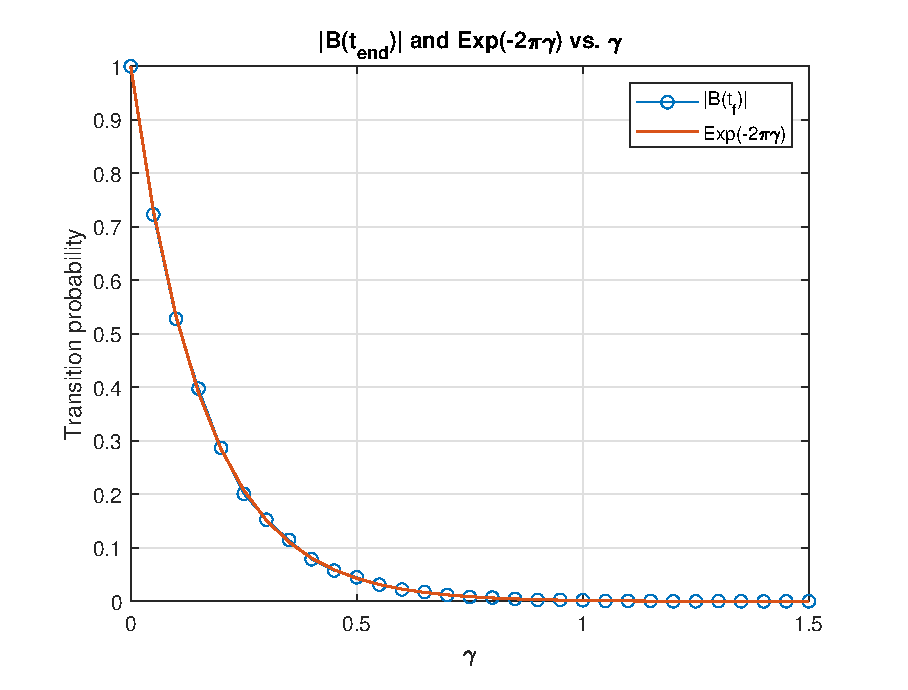
\includegraphics[width=\textwidth]{t200.eps}
		\caption{$\tau\in [-200,400]$}
		\includegraphics[width=\textwidth]{t400.eps}
		\caption{$\tau\in [-400,400]$}
	\end{minipage}
	\caption{$\abs{B(\tau)}^2$ approaches $\exp(-2\pi\gamma)$ as the $\tau$ goes to $\infty$. Here, $\gamma \in [0,1.5]$}
	\label{fig:tau_Infty}
\end{figure}


MATLAB code:
\begin{lstlisting}
% Huan Q. Bui
% Exponential decay in LZ transition probability

clear all
close all

% solve LZ ODE for these gammas
gamma = 0:0.05:1.5;
tspan = [-50 50];
B0 = 1;
C0 = 0;

B_list = [];

for g = gamma
[t,y] = ode45(@(t,y) LZ_ODE(t,y,g),tspan,[B0; C0]);
% y(1) = B
% y(2) = C = \dot{B}

% append the last B(t) = B(t=end) to B_list
B_list = [B_list abs(y(end,1))^2];
end


plot(gamma,B_list,'-o')
hold on
plot(gamma, exp(-2*pi*gamma), 'LineWidth', 1)
hold off
title('|B(t_{end})| and Exp(-2\pi\gamma) vs. \gamma')
xlabel('\gamma')
ylabel('Transition probability')
legend('|B(t_f)|', 'Exp(-2\pi\gamma)')
grid on

function dydt = LZ_ODE(t,y,g)
dydt = [y(2); -1i*g.*t.*y(2) - g^2.*y(1)];
end

\end{lstlisting}



\bibliography{BUI_LandauZener} 
\bibliographystyle{unsrt}	

\end{document}